\chapter{Phase Transition, Critical Phenomenon \& Renormalized Group}

\section{Categories of Phase transitions}

\begin{enumext}[]
  \item 1 order: At the phase transition point,
  the chemical potential of the two phases are equal,
  but the partial derivation is not equal, that is
  \begin{equation}
    \mu^a - \mu^b = 0, \qq{and}
    \rho_a \neq \rho_B (= \pdv NV),
    S^a - S^b = -\ab(\pdv{\mu^a}T)_P + \ab(\pdv{\mu^b}T)_P \neq 0.
  \end{equation}
  \item 2 order: $\Delta\mu = 0$, $\Delta S = 0$, $\Delta \rho = 0$.
  But the heat capacity $\pdv[2]\mu T$, expansion factor $\pdv\mu{T,\beta}$,
  and the compression factor $\pdv[2]\mu p$ are not continuous.
  $\Delta C_p \neq 0$, $\Delta$, $\Delta k \neq 0$
  \item 3 order: BEC is advanced
  (without $K-T$ phane transition, 1 order or $\infty$ order)
\end{enumext}

\section{Landau 2 order phase transition theory}

描述相变:序参量, 对称性破缺

序参量:用于区分两个相不同的物理量. 例如:磁性物质中,有顺磁(磁化强度 $M = 0$),铁磁(磁化强度 $M \neq 0$).

$M = \sum (-1)^i s_i$

[!Figure] 顺磁 [!Figure] 铁磁 \textrightarrow SU(2) Conservatioin.

随 $T \downarrow$ 的相变,叫自发对称破缺.

自发破缺和序参量
\begin{enumext}
  \item 固液相变,平移不变性 用 DLRO 参数表示.
  \item 液体--液晶:转动对称性,密度的各向异性.
  \item 超导 -- Normal Metal: 基态粒子数守恒.
  序参量:$|\text{电子对 (Copper pair)}\text{波函数}|^2$.
  \item Boson 超流:$k = 0$ 粒子数守恒 \textrightarrow\ ODLRO.
  \item 二元合金固体结构相变:晶体点群 $\frac{W_1 - W_2}{W_1 + W_2}$
\end{enumext}

\begin{definition}[序参量]
  序参量概念也用到一级相变.
\end{definition}
气 --- 液相变:一级相变,$\rho_\text{liquid} - \rho_\text{gas} = 0$.

外磁场中的超导 --- NM 相变 $|\text{超导波函数}|^2$

理想波色紫超流:三级相变. $k = 0$, 波色紫密度.

\subsection{Gingbang-Landau}

The Gibbs free energy of Superconductor,
as a function of SC order parameter $\psi$.

At the critical point
\[
  g_s(\psi = 0) = g_n
\]
and
\[
  g_s(\psi) = g_n + A|\psi|^2 + \frac B2|\psi|^4 + \cdots
\]
when $T < T_c$, $g_s < g_n$, and $A(T) < 0$ ($A(T_c) = 0$).
then, around $T_c$
\[
  A(T) = (T - T_c) \ab(\pdv AT)_{T=T_c}
\]
while $B = \text{Const}$, $B(T) = B(T_c) = B_c$.
\[
  \odv{g_s(\psi)}\psi = 0, \quad A + B_c|\psi|^2 = 0
\]
then we have $|\psi|^2 = -A/B_c$, $g_s = g_n - A^2/2B_c$.
On the other hand,
\[
  g_n - g_s = \mu_0H_c^2(T)/2
\]
around $T_c$,
\[
  H_c^2(T) = \frac{A^2}{\mu_0B_c} = \frac{(T_c - T)}{\mu_0B_c}\ab(\pdv AT)_{T = T_c}, \quad
  H_c \propto T_c - T
\]
In Landau's theory, $GL$: $|\psi|^2 = n_s$ should has a space distribution
\[
  g_s = g_n + A|\psi|^2 + \frac B2|\psi|^4 + \frac1{2n^*}|-\iu\hbar\nabla\psi|^2
\]
while $\psi$ is the pairing function. the second term becomes
\[
  |(\iu\hbar\nabla - e^* \bm A)\psi|
\]
where $e^* = 2e$.
\[
  \fdv{G_s}{\varphi^\alpha} = 0 \Rightarrow
  \begin{cases*}
    A\psi + B|\psi|^2\psi - \frac{\hbar^2}{2m^*}D^2\psi = 0\\
    \hat n \cdot D\psi = 0, & 
  \end{cases*}
\]
Consider weak field $|\bm A\psi| \gg |\Delta\psi|$.
Then ignore $\bm A$, $\psi_0 = \sqrt{|A|/B}$.
$\psi \sim \psi_0$, $f = \frac\psi/\psi$, $f^* = f$.
then we have
\[
  -\frac{\hbar^2}{2m_c^*A} \nabla^2f + f - f^3 = 0.
\]
To summarize
\begin{align}
  \begin{cases}
    \xi^2\odv[2]f\xi + f - f^3 = 0\\
    f(0) = 0, ~\pdv fz|_{z\to0} = 0\\
    f'(\infty) = 1, ~\pdv fz_{z\to\infty} = 1.
  \end{cases}
\end{align}
\[
  \int_{\infty}^z \d x \xi^2 \ab(\odv fz)
  \odv*{\ab(\odv fz)}z
= \int_{\infty}^z \d z \odv*{\ab(\frac14 f^4 - \frac12 f^2)}z
\]
Expand it
\[
  \frac12 \xi^2 \ab(\odv fz)^2 = \frac14f^4 - \frac12f^2 + \frac14
= \frac12(1 - f^2)^2
\]
Since $\odv fz > 0$,
\[
  \odv fz = \frac{1 - f^2}{\sqrt2\xi(T)},\quad
  f = \tanh \frac{z}{\sqrt2 \xi(T)}
\]
where
\[
  \xi(T) = \frac{\hbar}{[2m^2 (T_c-T)\pdv A{T_c}]^{1/2}} \to \infty,
  \quad T \to T_c
\]
The coherent long wave divergent at the critical point.

\section{Critical Phenomenon and Critical Index}

At critical point, $\xi \propto (T_c - T)^{-1/2}$.

Physics parameters behave the dependence of the power function of $\Delta T$ at the critical point, it's the so-called critical phenomenon.
The power exponents are the critical exponents.
$\alpha$, $\beta$, $\gamma$, $\delta$, $\nu$, $\eta$
stands for different physics parameters.

Since $f$ is the function of $\epsilon = \frac{T-T_c}{T_c}$,
that is
\[
  f(\epsilon) = \epsilon^\lambda (1 + B\epsilon^\lambda), ~
  \lambda > 0
\]
$\lambda = \lim_{\epsilon\to0} \frac{\ln f(\epsilon)}{\ln \epsilon}$
is the critical exponent.
\begin{enumext}[label = (\alph*)]
  \item $\beta$: The order parameter, which is decided with the change of temperature.
  $M(T) \propto (T - T_C)^\beta$
  \begin{itemize}
    \item Superconductivity: $|\psi| \propto (T - T_c)^{1/2}$
    \item Gas \& liquid phase transition: $\Delta\rho \propto (T_c - T)^\beta$, $T \to T_c^-$, $p = p_c$.
    The order parameter $\sim |T - T_c|^\beta$.
  \end{itemize}
  \item The flatness of critical isotherms $\delta$
  \[
    H = M^\delta \sgn(M) \quad(T \to T_c,~ H \to 0)
  \]
  while
  \begin{gather}
    (p - p_c) \sim |\rho - \rho_c|^\delta \sgn(\rho - \rho_c), \quad(T = T_c, p \to p_c)\\
    (H - H_c) \sim |\psi|^\delta ~ (T = T_c)
  \end{gather}
  \item $\chi_0$, $K_t$, $\gamma$
  \begin{gather*}
    X_0 = \ab(\pdv MT)_T \bigg|_{H\to0}
    \text{Suspetibility, zero field magnetic ratio}\\
    X_0 \sim (T - T_c)^{-\gamma}\\
    K_T = -\frac1V \ab(\pdv V\beta)_T \text{is isotherm compress ratio}\\
    K_T \sim (T - T_c)^\gamma, ~ (T \to T_c, ~ p \to p_c)
  \end{gather*}
  \begin{framed}
    \[
      \pdv{\text{Order parameter}}{\text{Extra field}}\bigg|_{\text{Extra field} \to 0} \sim (T - T_c)^{-\gamma}
    \]
    is so-called zero-field response.
  \end{framed}
  \item Heat capacity $\alpha$
  \begin{itemize}
    \item Magnetic: $C_H \sim (T - T_c)^{-\alpha}$, $H \to 0$
    \item Liquid: $C_V \sim (T - T_c)^{-\alpha}$, $T \to T_c$, $p = p_c$
  \end{itemize}
  \item Correspond length $\nu$
  $A(\bm r,t)$, $B(\bm r,t)$
  \[
    \braket<(A(\bm r,t) - \braket<A>)(B(\bm r,t) - \braket<B>)>
  \]
  is called the correspond function between $A$ and $B$.
  \[
    \braket<(S_i - \braket<S_i>) (S_j - \braket<S_j>)>
  \]
  $A = B$, $\bm r = \bm r'$, $t = t'$
  \[
    G(r,t) = \braket<(A(\bm r,t) - \braket<A>)^2> = \braket<A^2(\bm r,t)> - \braket<A>^2
  \]
  is called raise and fall.
  
  MFA: $G(r) \sim \frac1r \upe^{-r/\xi}$,
  $\xi$ is called the correspond length.
  At the critical point, $\xi \sim |T - T_c|^{-\nu}$.
  \[
    f = \tanh \frac{\delta}{\sqrt2\xi(T)},
    f - 1 \sim \upe^{-\frac{\gamma}{\sqrt2\xi}}
  \]
  For superconduct G-L equation, $\xi \propto |T - T_c|^{-1/2}$, $\nu = 1/2$.

  But MF estimation some times has difference from the experient result.
  \item Correspond function
  \[
    G(r) \sim r^{-d+2-\eta},~ d = \text{space dimesions}
  \]
  it should be a power law.
  After taking the Fourier transformation,
  \[
    G(k) \sim k^{\eta-2}
  \]
\end{enumext}
\begin{itemize}
  \item These critical exponents can be measured in experients.
  \item Since the raises and falls around the critical point is large, it will take longer time to reach equilibrium (临界慢化)
  \item The accuracy of the measure is not good (P. 480, Lin).
\end{itemize}
These critical exponents have the relations: scaling law (标度律).
\begin{align}
  \alpha + 2\beta - \gamma = 2\\
  \gamma = \beta(\delta - 1)\\
  \gamma = \nu(2 - \eta)\\
  \nu d = 2 - \alpha
\end{align}
There are $6 - 4 = 2$ independent variables.
这些关系与具体的微观细节无关,具有一定的普适性(普适性假设).

The critical behaviors of the system is determined by two variables:
One is the dimension of space $d$, and the dimesion of the order parameter $n$.
If $d = n$, the critical phenomenons are included in the same 普适类.

The order parameters of a system can be real number, complex number, or vector.
If it's 实数, then $n = 1$; if it's complex number, then $n = 2$.
For 3D space vector, $n = 3$.

\begin{itemize}
  \item $n = 1$, 气液相变密度差二元合金中,占位率差.
  \item $n = 2$, XY model, wave functions in superflow and superconduct.
  \item $n = 3$, Heisenberg model
\end{itemize}
The physics behind 普适性:The correspond length will be infinity at the critial point.

\section{Quantum Phase Transition}

Quantum Phase Transition is at the temperature of $T = 0$,
the different phases of the system occur phase transition
due to the change of some parameter.

For a finite system, assume $H(g)$ is Hamiltonian, $g$ is coupling constant.
Usually, $E(g)$ is the smooth function of $g$, means that no phase transition.

Sometimes
\[
  H = H_0 + gH,
\]
where $[H_0, H_1] = 0$.
Then, $H_0$, $H_1$ can be diagnosed at the same time, and they have the common eigenfunction
\[
  E_n = E_n^{(0)} + gE_n^{(1)}
\]
$E_0 = E_0^{(0)} - gE_0^{(1)}$, $E_0 = E_1^{(0)} - gE_1^{(1)}$.
At $g = g_c$, $E_0(g_c) = E_1(g_c)$, $g_c = \frac{E_1^{(0)} - E_0^{(0)}}{E_0^{(1)} - E_1^{(1)}}$.
\[
  E_1 = 1 + g3,~ E_0 = 1 + g(-2) \Rightarrow g_c = -\frac15
\]
Since $[H_0, H_1] \neq 0$. For infinite lattice system, will have the second condition,
\begin{enumerate}
  \item Simple level crossing: 1st level phase transform
  \item The opened $g^a$ is infinite near to zero, then quantum phase transformation will take place. The correction function will have difference on 定性 before and after phase transition.
  
  The quantum phase transition take place at the energy gap $\Delta \to 0$, or the 元激态 on the basis state.
  \[
    \Delta \sim J|q - q_c|^{Z\nu}
  \]
  \begin{enumerate}
    \item $k_BT < \Delta$. quantum fluctuanctism will stronger than the heat fluctuanctism.
    Quantum critical
    \item $k_BT < \Delta$. quantum fluctuanctism will weaker than the heat fluctuanctism.
  \end{enumerate}
\end{enumerate}

\section{Ising Model}

Hamiltonian
\[
  H = -J \sum_{<ij>} S_i^z S_j^z - B\sum_i S_i^z
\]
where $S_i^z = \pm\frac12\hbar$, $S_i^z \to \sigma_i = \pm1$

\subsection{Average field approximation}

Hamiltonian
\[
  H = -\sum_i \sigma_i (B = J \sum_\delta S_{i+\delta})
\]
Replace $\sigma_{i+\delta}$ with $\bar\sigma = \braket<\sigma_{i+\delta}>$,
$\sum_\delta\bar\sigma = z\bar\sigma$. Now,
\[
  H_{MF} = -\sum_i (B + \bar h)\sigma_i
\]
where $\bar h = zJ\bar\sigma$. Then
\begin{align*}
  Z_{\parallel} = & \sum_{\sigma_1} \cdots \sum_{\sigma_N}
    \exp\ab[\sum_i \beta(B + \bar h) \sigma_i]
  = \sum_{\sigma_1} \exp\ab[\beta(B + \bar h)\sigma_1]
    \sum_{\sigma_2} \exp\ab[\beta(B + \bar h)\sigma_2]\\
  = & \prod_i \ab(\sum_{\sigma_i} \exp\beta(B + \bar h)\sigma_i)
  = \prod_i \ab[\exp \beta(B + \bar h) - \exp\ab[-\beta(B + \bar h)]]
  = \ab[2\cosh\ab(\frac{B + \bar h}{k_BT})]^N
\end{align*}
and
\begin{gather*}
  F = -k_BT \ln Z_N
= -Nk_BT\ab\{\ln z + \ln \cosh\ab[\frac{B}{k_BT} + \frac{zJ}{k_BT}\bar\sigma]\}\\
  M = N\bar\sigma = -\pdv FB = N \tanh\ab(\frac{B}{k_BT} + \frac{zJ}{k_BT} \bar\sigma)
\end{gather*}
then we can obtain the expression of $\sigma$ (it's the 自洽方程 of $\sigma$).
\begin{itemize}
  \item If $B = 0$, then
  $\bar\sigma = \tanh\ab(\frac{ZJ}{k_BT} \bar\sigma) = \tanh\ab(\frac{T_c}{T}\bar\sigma)$, where $T_c = \frac{ZJ}{k_B}$
  Denote $y = \tanh\ab(\frac{T_c}{T}\bar\sigma)$, $u' = \bar\sigma$.
  Then we can plot $y(\bar\sigma)$: linear; Also $T > T_c$ and $T < T_c$.
  % \begin{tikzpicture}
  %   \addplot[domain = 0:360] {sin(x)};
  % \end{tikzpicture}
  $\bar\sigma = 0$ or $\pm\sigma_0$.

  In another way, $H(-\sigma_i) = H(\sigma_i)$, means $Z_2$ has the symmetry,
  leads to 自发破缺.

  $\sigma_0 = \sigma_0(T)$, $T \sim T_C^-$, $\bar\sigma_0 \sim 0$.
  \[
    \tanh \frac{T_c}{T}\bar\sigma \approx \frac{T_c}{T} \bar\sigma - \frac13\ab(\frac{T_c}{T}\bar\sigma)^3 = \bar\sigma
  \]
  then we obtain $\bar\sigma = \sqrt3\ab(1 - \frac T{T_c})^{1/2}$, and
  $M = N\bar\sigma \sim (T_c - T)^{1/2}$.
  \[
    C_B =
    \begin{cases}
      0,        & T \to T_c^+\\
      3Nk_BT_c, & T \to T_c^-
    \end{cases}
  \]
  Now $M \sim (T - T_c)^{-1} B$,
  $\chi = \pdv MB \sim (T - T_c)^{-1}$, $M(T_c,B) \sim B^{1/3}$.
  $\beta = \frac12$, $\alpha = 0$, $\gamma = 1$, $\delta = 3$,
  $T_c = \frac{zJ}{k_B}$, it's finite.
  \item If $B \neq 0$, then ...
\end{itemize}

\subsection{The exact solution of 1D Ising model}

The Hamiltonian
\[
  H = -J \sum_n \sigma_n \sigma_{n+1} - h\sum_n \sigma_n
\]
with a 1D chain, or a circle (Periodic Boundary Condition $N + 1 \equiv 1$)
\begin{center}
  \begin{minipage}{.48\linewidth}
    \centering
    \begin{tikzpicture}
      \draw (0,0) --++ (5,0);
      \foreach \i in {1,2,...,5}
        \draw ({\i - .5},-.1) --++ (0,.2) node [below = 1ex] {\ifnum \i<3 $\i$ \fi} node [below = 1ex] {\ifnum \i=5 $N$ \fi};
    \end{tikzpicture}
  \end{minipage}
  \hspace*\fill
  \begin{minipage}{.48\linewidth}
    \centering
    \begin{tikzpicture}
    \draw (0,0) circle (2);
    \foreach \i in {15,30,...,360}
      \draw (\i:1.9) --++ (\i:.2);
    \node [right, rotate around = {0:(0,0)}] at (0:2) {$n$}
     node [left, rotate around = {-15:(0,0)}] at (165:2) {$N$}
     node [left, rotate around = {0:(0,0)}] at (180:2) {$N + 1 \equiv 1$}
     node [left, rotate around = {15:(0,0)}] at (195:2) {$2$};
  \end{tikzpicture}
  \end{minipage}
\end{center}
The partition function is
\begin{equation}
  \begin{aligned}
Z & = \sum_{\sigma_1, \cdots, \sigma_N}
      \exp\{K \sum_n \sigma_n\sigma_{n+1}\}
      \exp\{B \sum_n \sigma_n\}\\
  & = \sum_{\substack{\{\sigma_n\}\\\{\sigma_n'\}}}
      \exp\{B\sigma_1\}\delta_{\sigma_1\sigma_1'}
      \exp\{K\sigma_1'\sigma_2\}
      \exp\{B\sigma_2\}\delta_{\sigma_2\sigma_1'}
      \exp\{K\sigma_2'\sigma_3\} \cdots
      \exp\{B\sigma_N\}\delta_{\sigma_N\sigma_N'}
      \exp\{K\sigma_N'\sigma_1\}
  \end{aligned}
\end{equation}
where $K = J/kT$, and $B = h/kT$.
We define $(V_1)_{\sigma_i\sigma_j} = \exp(K\sigma_i\sigma_j)$,
$\sigma_i = \pm1$, $\sigma_j = \pm1$ stands for two directrions of spins $\ket|\uparrow>$ and $\ket|\downarrow>$,
Conduct a $2 \times 2$ matrix.
Also for $(v_2)_{\sigma_i\sigma_j} = \exp(B\sigma_i) \delta_{\sigma_i\sigma_j}$.
The matrix can be expressed as
\begin{equation}
  V_1 = \begin{pmatrix}
    \upe^K & \upe^{-K}\\
    \upe^{-K} & \upe^K
  \end{pmatrix}, \qq{and}
  V_2 = \begin{pmatrix}
    \upe^B & 0\\
    0 & \upe^{-B}
  \end{pmatrix}
\end{equation}
so, we can express $Z$ in terms of the elements of matrices
\begin{equation}
  \begin{aligned}
  Z & = \sum_{\substack{\{\sigma_n\}\\\{\sigma_n'\}}}
        (V_2)_{\sigma_1\sigma_1'} (V_1)_{\sigma_1'\sigma_2} \cdots
        (V_2)_{\sigma_N\sigma_N'} (V_1)_{\sigma_N'\sigma_1}\\
    & = \Tr(V_2 V_1 \cdots V_2 V_1)
      = \Tr(V_2 V_1)^N = \Tr(V_2 V_1^{1/2} V_1^{1/2})^N
      = \Tr(V_1^{1/2} V_2 V_1^{1/2})^N = \Tr V^N
  \end{aligned}
\end{equation}
where
\begin{equation}
  V = \begin{pmatrix}
    \upe^{K+B} & \upe^{-K}\\
    \upe^{-K} & \upe^{K-B}
  \end{pmatrix} = \upe^{K+B}I + \upe^{-K}\sigma_x
\end{equation}
The eigenfunction
\begin{equation}
  \det(V - \lambda) = 0,~
  \lambda_\pm \upe^{K} \cosh B \pm \sqrt{\upe^{2K} \sinh^2B + \upe^{-2K}}
\end{equation}
Then, the trance to $V^N$ is
\begin{equation}
  \Tr(V^N) = \Tr\ab[
    \pdiagmat{\lambda_+,\lambda_-}^N
  ] = \lambda_+^N + \lambda_-^N
= \lambda_+^N[1 + (\lambda^-/\lambda_+)^N] \xrightarrow{N\to\infty} \lambda_+^N
\end{equation}
From the expension of $\lambda_+$, we have
\begin{equation}
  f = \frac FN = -\frac1{\beta^N} \ln Z = -\beta^{-1} \ln \lambda_+,\quad
  M \propto -\pdv fh = \beta^{-1} \frac{\partial \ln \lambda_+}{\beta^{-1} \partial B} = \sinh B(\sinh^2B + \upe^{-4K})^{1/2} \xlongrightarrow[T>0]{B\to0} = 0
\end{equation}
So, at a finite temperature, there's no phase transition, and the mean field
$T_c = 2J/k_B$. In summary,
\begin{equation}
  T = 0, \quad M = \frac{\sinh B}{\sinh B = 1}, \quad T_c = 0
\end{equation}

\subsection{2D Ising Model}

For $2D$ Ising model, $h = 0$ have exact solution. Now the matrix
\begin{equation}
  V = \begin{pmatrix}
    \upe^K & \upe^{-K}\\
    \upe^{-K} & \upe^K
  \end{pmatrix} = \upe^KI + \upe^{-K}\sigma_x
= \upe^{K}(I + \upe^{-2K}\sigma_x)
\end{equation}
we can define $\tanh a = upe^{-2K}$. Then
\[
  \exp(a\sigma_x) \ab(= \sum_{n=0}\frac1{n!}(a\sigma_x)^n)
= I\cosh a + \sigma_x \sinh a
\]
Then, we can define
\[
  V = A\exp(a\sigma_x) = A\cosh a(I + \tanh a \sigma_x)
= A \cosh a(I + \upe^{-2k} \sigma_x)
\]
And $A$ can be expressed as
\[
  A = \frac1{\cosh a \sqrt{\tanh a}}
= \frac1{\sqrt{\cosh a \sinh a}} = \sqrt{\frac2{\sinh 2a}}
\]
Since
\[
  \sinh 2a \sinh 2k = 2\sinh a\cosh a \ab(\frac1{\tanh a} - \tanh a)
= 2(\cosh^2 a - \sinh^2a) = 2, \qq{then}
A = \sqrt{\sinh 2k}, ~ F = \sqrt{\sinh 2k} \exp(a\sigma_x)
\]
We can draw the 2D lattice: $j = (1,2)$, $(2,3)$, $\cdots\,$,~$(N,1)$.
\begin{center}
  \begin{tikzpicture}[xscale = 2, yscale = .75]
    \draw (0,0) node [left] {$1$} --++ (4,0);
    \draw (0,1) node [left] {$2$} --++ (4,0);
    \draw (0,2.5) node [left] {$n-1$} --++ (4,0);
    \draw (0,3.5) node [left] {$n$} --++ (4,0);
    \draw (0,4.5) node [left] {$n+1$} --++ (4,0);
    \draw (.5,-.5) --++ (0,5.5) node [above] {$m-1$};
    \draw (2,-.5) --++ (0,5.5) node [above] {$m$};
    \draw (3.5,-.5) --++ (0,5.5) node [above] {$m+1$};
  \end{tikzpicture}
\end{center}
Consider fixed the $m-th$ column, $V \to V(m,j) = \sqrt{\sinh 2k_1} \exp(a \sigma_j^{x^{(m)}})$; The Ising model for this column is
\begin{gather}
  H = -J \sum_{m,n} \sigma_{mn} \sigma_{m,n+1} - J_2 \sum_{m,n} \sigma_{mn}\sigma_{m+1,n},\\
  Z = \sum_{\{\sigma_{m,n}\}} \exp\ab\Bigg(\underbrace{K_1 \sum_{mn}\sigma_{mn} \sigma_{m,n+1}}_{\prod_j V_1(j,m)} +
  K_2 \sum_{mn}\sigma_m \sigma_n \sigma_{m+1,n})
\end{gather}
and we can define $V_2(m)$
\begin{equation}
  V_2(m) \equiv \upe^{K_2 \sum_j \sigma_{m,j} \sigma_{m+1,j}} V(m)
= (\sinh 2k_1)^{N/2} \upe^{K_1 \sum_j \sigma_j^{x(m)}}
\end{equation}
In terms of trace
\[
  Z = \Tr(V_2^{1/2} V_1 V_2^{1/2})^M = \Tr V^M,
\]
where $V_2$ and $V_2$ are $2M \times 2M$ matrices, and
\[
  \{\sigma_i^a, \sigma_j^b\} = \delta^{ab}, \quad
  [\sigma_i^a, \sigma_j^b]_{i\neq j} = 0
\]
To make it behaves as fermion, we shall
\begin{gather}
  c_j =   \exp\ab(\pi\iu \sum_{l=1}^{j-1} \sigma_{l^+}\sigma_{l^-}) \sigma_j^-\\
  c_j^+ = \exp\ab(\pi\iu \sum_{l=1}^{j-1} \sigma_{l^+} \sigma_{l^-}) \sigma_j^+
\end{gather}
where $\sigma_i^\pm = \sigma_i^x \pm \iu\sigma_i^y$. Then we have
\begin{equation}
  \{c_j^+, c_{j'}\} = \delta_{jj'},\quad
  c_j^\dagger c_j = \sigma_j^\dagger \sigma_j^-
\end{equation}
which is so-called Jordan-Wigner Transmission.
To inverse, we have
\begin{equation}
  \sigma_{j^+} = \exp\ab(\iu\pi\sum_{l=1}^{j-1} c_l^\dagger c_l) c_j^\dagger,\quad
  \sigma_j^- = \exp\ab(\iu\pi\sum_{l=1}^{j-1} c_l^\dagger c_l) c_j
\end{equation}
We make a transformation in $V_1$, and $V_2$
\begin{equation}
  (\sigma_x,\sigma_y,\sigma_z) \to
  (\sigma_x',\sigma_y',\sigma_z') = (-\sigma_z,\sigma_y,\sigma_x)
\end{equation}
i.e., $\sigma_x\sigma_y = \iu\sigma_z \to \sigma_x'\sigma_y' = \iu\sigma_z'$.
Then,
\begin{equation}
  V_1 = (\sinh 2K_1)^{M/2} \exp\ab[-2K_1 \sum_j\ab(\sigma_{j^+} \sigma_{j^-} - \frac12)]
= (\sinh 2k_1)^{M/2} \exp\ab[-2K_1 \sum_j\ab(c_j^\dagger c_j - \frac12)]
\end{equation}
In $V_2$, make the transformation $\sigma_z \to \sigma_x = \sigma_+ - \sigma_-$,
Then
\begin{equation}
  V_2 = \exp\ab\{K_2 \sum_{j=1}^{M-1} (c_j^\dagger - c_j)(c_{j+1}^\dagger + c_{j+1})
  - (-1)^{\hat n} (c_M^\dagger - c_M) (c_1^\dagger - c_1)\}
\end{equation}
where $\hat n = \sum_{l=1}^M c_l^\dagger c_l$.
Now,
\begin{equation}
  \frac FN = -\beta^{-1} \ab[\ln(2\sinh 2K_1)^{1/2} + \frac1{4\pi} \int_{-\pi}^\pi \epsilon_q \d q]
\end{equation}
where
\[
  \cos \epsilon_q = \cosh 2K_2 \cosh 2a - \sinh2K \sinh2a \cos q
\]
Since $\sinh 2a = \sinh 2K_2$ is fixed, then $J_1 = J_2$.
The critial temperature now satisfies
\begin{equation}
  \frac{k_BT_c}{J} \approx 2.7 \neq 0
\end{equation}
The heat capacity ratio 
\begin{gather}
  C \propto \ln\ab|1 - \frac T{T_c}|,\\
  M \propto \begin{cases}
    (1 - T/T_c)^{1/8}, & T < T_C,\\
    0, & T > T_c,
  \end{cases}\\
  g(r) \sim \begin{cases}
    (T - T_c)^{1/4} \frac{\upe^{-r/3}}{(r/3)^{1/2}}, & T > T_c,\\
    (T_c - T)^{1/4} \frac{\upe^{-2r/3}}{(r/3)^{1/2}}, & T < T_c,
  \end{cases}\\
  \chi \sim |t|^{-7/4}, ~ t = (T - T_c)/T_c ~ \xi \sim (T - T_c)^{-1}.
\end{gather}
To compare with the exact solution,
\begin{center}
  \begin{tabular}{*7l}
    \toprule
    Exact Solution & $\alpha = 0$ ($\ln$) & $\beta = 1/8$ & $\gamma = 7/4$ &
    $\nu = 1$ & $\eta = 1/4$ & $\delta = 15$\\
    \midrule
    MF & $\alpha = 0$ (discontinuation) & $\beta = 1/2$ & $\gamma = 1$ &
    no $\nu$ & no $\eta$ & $\delta = 3$\\
    \bottomrule
  \end{tabular}
\end{center}

\subsection{1D + 1D dimensional quantum Ising model}

Which is so-called the Horizontal field Ising model, in a chain.
The Hamiltonian is
\begin{equation}
  H = -K \sum_n \sigma_n^z \sigma_{n+1}^z - \bm h \cdot \sum_n \bm \sigma_n
\end{equation}
where $\bm h = (h_x, 0, 0)$, $\bm \sigma = (\sigma_x, \sigma_y, \sigma_z)$.
Obviously, $[\sigma^z, \sigma^x] \neq 0$.
We shall prove that \emph{1D + 1D quantum Ising model is equivalent to 2D Ising model}.
\begin{proof}
  Starting from the 0D + 1D single spin model is equivalent to 1D Ising model
  \[
    Z_{1D} \longleftrightarrow \Tr \upe^{-H_Q/kT},~
    H_Q = -h_x\sigma_x
  \]
  and $M$ site lattice ($K_1$).
  \begin{align}
    V & = V_1 = \upe^{K_1} (1 + \upe^{-2K_1} \sigma^x)
  = \sqrt{\frac{M}{\beta h_x}} \ab(1 + \frac{h_x\beta}{M})\\
    V^M = \ab(\frac M{\beta h_x})^{M/2} (1 + \frac{h_x\beta}{M} \sigma^x)^M
  = & \ab(\frac M{\beta h_x})^{M/2} (1 - \Delta \tau H_Q)^{\beta/\Delta\tau}
  \xlongequal{\Delta\tau \to 0} \ab(\frac M{\beta h_x})^{M/2} \upe^{-\beta H_Q}
  \end{align}
  where $\Delta\tau = \beta/M$.
  When $M \to \infty$,
  \begin{equation}
    Z_{1D} = \Tr V^M = \Tr \upe^{-\beta H_Q}
  \end{equation}
  For 2D Ising model, the $n$-th chain
  \begin{equation}
    V_n(j) = \sqrt{\frac M{\beta h_x}}\ab(1 + \frac{h_x\beta}{M} \sigma_n^x), \quad
    V_n^M = \ab(\frac{M}{\beta h_x})^{M/2} \upe^{-\beta h_Q(n)}
  \end{equation}
  Concering the couple between chains,
  \begin{align*}
    \exp\ab(K_i \sum_{m,n} \sigma_{m,n}^z \sigma_{m,m-1}) &
  = \prod_m \exp\ab(K_2 \sum_n \sigma_{m,n}^z \sigma_{m, n+1}^\delta)\\
  & \approxeq \exp\ab(\frac{K_2}{\Delta \tau}\beta \sum_n \sigma_n^z \sigma_{n+1}^z)
  \equiv\exp(\beta K \sum_n \sigma_n^z \sigma_{n+1}^z)
  \end{align*}
  So, we obtain the Horizontal field 2D Ising model
  \begin{equation}
    H_\text{2D} = \ab(-K \sum_n \sigma_n^z \sigma_{n+1} - h_x \sum_n \sigma_n^x)
  \end{equation}
  Now, back to the proof. We have
  $h\Delta\tau = \upe^{-2K_2}$, $K\Delta\tau \equiv K_\tau$.
  At the critial point, $\sinh 2K_x \sinh2K_\tau = 1$,
  or $\frac{2K\Delta\tau}{2h\Delta\tau} = 1$, then we have $K = h$.
  \begin{equation}
    \begin{cases*}
      K = h, & QCP\\
      K > h, & FM\\
      K < h, & Quantum disorder
    \end{cases*}
  \end{equation}
  The Quantum 1 + 1 Ising model (such as 2D) Lagrangian is
  \begin{equation}
    \psi \bar\psi + \bar\psi \partial\bar\psi
  \end{equation}
  which is very simple, where $\partial = \pdif x - \iu\pdif y$, $\bar\partial = \pdif x + \iu\pdif y$, and $\bar\partial \psi = 0$, $\partial \bar\psi = 0$.
\end{proof}

\section{Renormalization Group}

\paragraph{Basic Point}

\begin{enumext}
  \item 作``粗粒化''尺度变换,RG is a ``half-group'' (No inverse element), 找出 RG 规律.
  \item Determine the ``fixed-points'', find the fixed-points that concerning to the critial points.
  \item Linearization the RG transformation, determine the critial index.
\end{enumext}

\subsection{Real space RG}

For the Spin model: $d$-space dim.
Treat the integral $l^d$ spins as a spin, i.e., for $l = 2$, $d = 2$,
\[
  \sigma: \begin{bmatrix}
    \uparrow & \uparrow\\
    \uparrow & \uparrow
  \end{bmatrix} \Longrightarrow \sigma': \uparrow
\]
$\sigma \to \sigma' = \pm 1$.
Then the previous $N$ sites becomes current $N = l^{-d}N$ sites.

For the spins, let $l = 2$, $d = 2$.
\[
  \begin{pmatrix}
    \begin{bsmallmatrix}
      \uparrow & \uparrow\\
      \downarrow & \downarrow
    \end{bsmallmatrix} &
    \begin{bsmallmatrix}
      \uparrow & \downarrow\\
      \downarrow & \uparrow
    \end{bsmallmatrix} &
    \begin{bsmallmatrix}
      \downarrow & \downarrow\\
      \uparrow & \uparrow
    \end{bsmallmatrix}\\
    \begin{bsmallmatrix}
      \uparrow & \downarrow\\
      \downarrow & \uparrow
    \end{bsmallmatrix} &
    \begin{bsmallmatrix}
      \downarrow & \downarrow\\
      \downarrow & \uparrow
    \end{bsmallmatrix} &
    \begin{bsmallmatrix}
      \uparrow & \uparrow\\
      \downarrow & \downarrow
    \end{bsmallmatrix}\\
  \end{pmatrix}
\]
At the beginning, $N = 24$, then $N' = 2^{-2} N = 24/4 = 6$.
\[
  \begin{cases}
    \begin{bsmallmatrix}
      -1 & -1\\
      -1 & 1
    \end{bsmallmatrix}~
    \begin{bsmallmatrix}
      -1 & -1\\
      1 & 1
    \end{bsmallmatrix}~
    \begin{bsmallmatrix}
      1 & 1\\
      1 & 1
    \end{bsmallmatrix} & \sigma' = 1\\
    \begin{bsmallmatrix}
      -1 & 1\\
      1 & 1
    \end{bsmallmatrix}~
    \begin{bsmallmatrix}
      1 & -1\\
      -1 & -1
    \end{bsmallmatrix} & \sigma' = -1
  \end{cases}
\]
Using the decimation (消元法)
\begin{equation}
  Z = \sum_{\{\sigma_i\}} \exp\ab[-\beta H_N(\sigma_i)]
\end{equation}
to let spins' degrees of freedom on the the $N - N'$ sites summed,
then
\begin{equation}
  Z = \sum_{\{\sigma_i'\}} \exp\ab[-\beta H_{N'}(\sigma_i)]
    = Z
\end{equation}
Assume $H_N$ is a 1D Ising model.
$i = 1$, $2$, $\ldots\,$,~$N$ = $1$, $3$, $5$, $\ldots\,$,~$2$, $4$, $\ldots\,$,~$6$. Then sum all the odd blocks.
If the free energies at the critial point are equal in two systems,
\[
  N'f^{(s)}(t',h') = Nf^{(s)}(t,h), \quad N' = Nl^{-d}
\]
where $t = (T - T_c)/T_c$, and $h$ is the external field.
\[
  f^{(5)}(t,h) = l^{-d} f^{(5)}(t,h)
\]
where $t$, $t'$, $h$, $h'$ are all small.
So the linear part
\[
  t' = l^{y_t}t, \quad
  h' = l^{y_h}h
\]
According to Scaling assumption, $f$ is not sensitive to scaling.
$f$ should be a function of the following variables that have no relation $l$
\[
\frac{h'}{|t'|^{y_h/y_t}} = \frac{h}{|t|^{y_h/y_t}} = \frac{h}{|t|^\Delta}
\]
At the same time, to cancel $l^{-d}$, $f^{(s)}$ should have the expression
\[
  f^{(s)}(t',h') = |t'|^{d/y_t} \tilde f(h/|t|^\Delta)
= l^{-d} |t'|^{d/y_t} \tilde f(h/|t|^\Delta)
= l^{-d} |l^{y_t} t|^{d/y_t} \tilde f(h/|t|^\Delta)
= |t|^{d/y_t} \tilde f(h/|t|^\Delta)
\]
If these can be achieved, then
\begin{align*}
  C_n & = \pdv[2]{f^{(s)}}t \sim |t|^{-(2-d/y_t)} \Rightarrow \alpha = 2 - \frac d{y_t}\\
  \frac MN & = \pdv{f^{(s)}}h = |t|^{d/y_t} |t|^{-\Delta} \odv*{\tilde f(h/|t|^\Delta)}{(h/|t|^\Delta)} \sim |t|^{d/y_t - \Delta}\\
  \pdv MH & = \pdv[2]{f^{(s)}}h \sim |t|^{d/y_t-2\Delta}
\end{align*}
where $\beta = \frac{(d - y_h)}{y_t} = 2 - \alpha - \Delta$,
$\gamma = \frac{2y_h-d}{y_t} = -(2\alpha - 2\Delta)$,
$\gamma = \beta(\delta - 1)$, $\delta = \frac\Delta\beta = y_h/(\alpha - y_h)$,
$\gamma = \beta(\delta - 1)$.
The correlation length $\xi' = l^{-1}\xi$.
We also want
\[
  \xi \sim |t|^{-\nu}, \quad \xi^\nu \sim |t'|^{-\nu}, \quad
  l^{-1} = (\xi'/\xi) = (t'/t)^{-\nu}, \quad \nu y_t = 1, \quad \nu = 1/y_t
\]
Then, $d \cdot \nu = d/y_t = 2 - \alpha$.
The Green function
\begin{align*}
  g(r') & = \braket<\sigma'(\bm r_1') \sigma'(\bm r_2')> \sim r_{12}'^{-(d+2-\eta)},\\
  g(r) = \braket<\sigma(\bm r_1) \sigma(\bm r_2)> \sim r_{12}^{-(d+2-\eta)}
\end{align*}
So, $\sigma'(\bm r') = l^{(d+2-\eta)/2} \sigma(\bm r)$,
$\gamma = (1 - \eta)^\nu$, $\eta = d + 2 - 2y_h$, $\sigma'(\bm r') = l^{y_h} \sigma(\bm r)$, i.e.,
$\sigma$ and $h$ has the same rescaling.

\subsection{Examples: 1D Ising model}

\begin{example}[Exponents (Exact result in \emph{Pathria's book})]
  \[
    Z = \sum_{\{\sigma_i\}} \exp\ab[\sum_{i=1}^N \ab(K_0 + K \sigma_i \sigma_{i+1} + \frac B2(\sigma_i + \sigma_{i+1}))]
  \]
  where $K_0 = 0$, $K = \beta J$, $B = \beta h$. Then the exponent
  \[
    \exp[\ldots] = \prod_{j=1}^{N/2} \exp[2K_0 + K(\sigma_{2j-1}\sigma_{2j} + \sigma_{2j}\sigma_{2j+1}) + \frac12B(\sigma_{2j-1} + 2\sigma_{2j} + \sigma_{2j+1})]
  \]
  where $\sigma_{2j} = \pm 1$.
  Then sum over $\sigma_{2j}$
  \begin{align*}
    &\prod_{j=1}^{N/2} \ab\{
      \exp\ab[2K_0 + K(\sigma_{2j-1} + \sigma_{2j+1})
    + \frac12B(\sigma_{2j-1} + \sigma_{2j+1} + 2)]
    + \exp\ab[2K_0 - K(\sigma_{2j} + \sigma_{2j+1}) + \frac12 B(\sigma_{2j-1} + \sigma_{2j+1} -2)]
    \}\\
  = & \prod_{j=1}^{N/2} \exp\ab[2K_0 + \frac12 B(\sigma_{2j-1} + \sigma_{2j+1})] \cdot 2\cosh(K(\sigma_{2j-1} + \sigma_{2j+1}) + 3)
  \end{align*}
  Do the transformation
  $\sigma_{2j + 1}$, $j = 0$, $1$, $2$, $\ldots \longrightarrow \sigma_j'$.
  \[
    Z = \sum_{\{\sigma_j'\}} \prod_{j=1}^{N/2} \exp(2K_2) 2\cosh(K(\sigma_j' + \sigma_{j+1'}) + B)\exp\ab[\frac12B(\sigma_j' + \sigma_{j+1}')]
  \]
  If we require $Z$ is still Ising model, then
  \[
    Z = \sum_{\{\sigma_j'\}} \exp\ab\{\sum_{j=1}^{N/2}\ab[K_0' + K'\sigma_j'\sigma_{j+1}' + \frac12B'(\sigma_j' + \sigma_{j+1}')]\}
  \]
  What are $K_0'$, $K'$, and $B'$?
  \begin{enumext}
    \item $\sigma_j' = \sigma_{j+1}' = 1$
    \[
      \exp(K_0' + K' + B') = \exp(2K_0 + B)2\cosh(2K + B)
    \]
    \item $\sigma_j' = \sigma_{j+1}' = -1$
    \[
      \exp(K_0' + K' - B') = \exp(2K_0 - B)2\cosh(-2K + B)
    \]
    \item $\sigma_j' = \sigma_{j+1}' = \pm1$
    \[
      \exp(K_0' - K') = \exp(2K_0)2\cosh B
    \]
  \end{enumext}
  Define $\exp(K_0') = \alpha$, $\exp K' = y$, $\exp B' = z$. Then,
  \begin{align*}
    xyz & = 2\exp(2K_0 + B)\cosh(2K + B)\\
    xy/2 & = 2\exp(2K_0 - B) \cosh(-2K + B)\\
    x/2 & = 2\exp(2K_0) \cosh B\\
    \upe^{K_0'} & = x = 2\upe^{2K_0}[\cosh(2K + B) \cosh(2K - B) \cosh^2B]^{1/4}\\
    \upe^{K'} & = y = [\cosh(2K + B) \cosh(2K - B)/\cosh^2B]^{1/4},\\
    \upe^{B'} & = z = \upe^B[\cosh(2K + B)/\cosh(2K - B)]^{1/2}
  \end{align*}
  Starting at
  \[
    Z_N(K,B) = \upe^{N'K_0'} Z_{N'}(K',B')
  \]
  where $K_0 = 0$.
  \begin{align}
    K' & = \frac14 \ln[\cosh(2K + B) \cosh(2K - B)] - \frac12\ln\cosh B
    \equiv R_K(K,B),\\
    B' & = B + \frac12\ln[\cosh(2K + B)/\cosh(2K - B)] \equiv R_B(K,B)
  \end{align}
  which is so-called RG equations.

  At the fixed points
  \[
    R_K(K^*,B) = K^*, \quad R_B(K^*,B^*) = B^*
  \]
  When $K^* = 0$, for any $B$, it is fixed point.
  The zero-interaction or $T \to \infty$.
  For another, $K^* \to \infty$, $B^* = 0$.
  Let $h = 0$, then $T \to 0$.

  Around the fixed point of $T \to 0$,
  \begin{align*}
    K' & = \frac12 \ln\cosh 2K \approxeq \frac12 \ln e^{2K}/2 = K - \frac12\ln 2,\\
    B' & \approxeq B + \frac12\ln\upe^{2B} = 2B
  \end{align*}
  Define $t = \exp(-\beta K)$, for $p > 0$.
  Then $t^* = 0$, $t' = 2^{p/2}t$.
  So, $l = 2$, $y_t = p/2$, $B' = 2B$, $y_h = 1$
  $\alpha = 2 - 2/p$, $\beta = 0$, $\gamma = 2/p$, $\delta = \infty$, $\eta = 1$.

  For normal situation, we can expand linearly at the fixed point to get the Linearization RG.
  For $n$ coupling constants, apply decimation
  \[
    N' = l^{-d} N, \quad \xi' = l^{-1} \xi, \quad l = 1, \quad
  \]
  For the vector $\bm K$
  \[
    \bm K' = R_l(\bm K), \quad
    \bm k^{(n)} = R_l (\bm K^{(n-1)}) = \cdots = R_l^n (\bm K^{(0)})
  \]
  when $n = 0$, $\bm K^{(0)} = \bm K$.
  Singular part of free energy per site
  \[
    f_s^{(n)} = l^{nd} f_s^{(n)}
  \]
  Now, the fixed point
  \[
    R_l(\bm K^*) = \bm K^*, \quad \xi(K^*) = l^{-1}\xi(K^*)
  \]
  then $\xi(\bm K^*) = 0$, or $\infty$. $P_\xi \sim \hbar \to P_\xi \to \infty$.
  \begin{itemize}
    \item $\xi(\bm K^*) = 0$, $P-\xi\to\infty$, is so-called ``UV'' fixed point, high energy.
    \item $\xi(\bm K^*) = \infty$, $P-\xi\to0$, is so-called ``inferred'' fixed point, low energy.
  \end{itemize}
  Around $K^*$,
  \begin{equation}
    K = K^* + \delta K, \quad
    K' = K^* + \delta K' = R_l(K^* + \delta K), \quad
    \delta K' = R_l(K^* + \delta K) - K^*
  \end{equation}
  Since $\delta K$ and $\delta k'$ are small,
  \[
    \delta K'_a = \ab(\odv{R_l}{K'}\bigg|_{K' = K*})_{ab}, \quad
    \delta K_b = (A_l^*)_{ab} \delta K_b
  \]
  where $A_l^*$ is the matrix that linearized from $R_l^*$.
  We can diagonalize $A_l^*$, then get the eigenvalues $\lambda_i$, and the eigenstates $\phi_i$
  \[
    \delta K = \sum_i u_i \phi_i, \quad
    \delta L' = \sum_i u_i A_l^* \phi_i = \sum_i u_i \lambda_i \phi_i
  = \sum_i u_i' \phi_i
  \]
  In a series of transformations, we have
  \[
    u_i^{(n)} = \lambda_i^n u_i^{(0)}
  \]
  \begin{enumext}
    \item If $\lambda_i > 1$, then $u_i \uparrow a = n$ gets more important. We call $u_i$ is relevant variabl. $\delta K'$ get more and more, and $K'$ gets far away from $K*$, then $K^*$ is unstable fixed point.
    \item If $\lambda < 1$, then $u_i$ is irrelevant variable, $K^*$ is stable fixed point.
    \item If $\lambda = 1$, then marginae variable logarithmic.
  \end{enumext}
\end{example}

\section{Numerical Renormalized Group \& DMRG}

\subsection{Momentum space renormalization}

For point-particle
\begin{equation}
  [x, p] \sim \hbar,
\end{equation}
when $p \to \infty$, then $\lambda \propto \frac1p$, i.e., \emph{UV radiation}.
The divergency (Singularity) need to be excluded\footnote{%
Normalization in QFT (actually, we cconsider QED).}, then an offsetting term
will be added for renormalization.

In momentum space, the ``scaling'' invariance ($\xi = 0$, $\xi \to \infty$).
The fixed point of $\xi = 0$ ($p \to \infty$, the fixed point of UV).

For the condensed matter, since $a = \text{finite}$, there is a ``natural''
cut-off, so we do not care about UV, but the infrared divergence
($p \sim \frac1L$), i.e., we consider the infrared fixed point
$\xi \to \infty$.

\subsection{Wilson's N.R.G.}

The basic concept of RG is, keep the states around the \emph{fixed point}, i.e.,
integrate or sum to ``cancel'' the unimportant states.

In the condensed matter, the important states include
\begin{enumerate*}
  \item the basic states,
  \item low-energy excited states.
\end{enumerate*}
Wilson
\begin{enumerate}
  \item Exactly diagonalize the $L$-sites subsystems (with Hamiltonian $H_L$)
  in a lattice system, with the observable variables $A_L$.
  \item After being exact diagonalied, take $n$ lowest energies $E_i$ and
  corresponging eigenstates $\psi_i$, ($i = 1$, $2$, $\ldots\,$,~$m$).
  \item Define $O_L = (\psi_1$, $\psi_2$, $\ldots\,$,~$\psi_m)$,
               $\bar H_L = O_L^\dagger H_L O_L
               \xlongequal{\text{diagonalization}}
               \pdiagmat*[empty = {}]{E_1, \ddots, E_m}$, similarly,
               $\bar A_L = O_L^\dagger A_L O_L = (\bar A_{ij})_{m\times m}$.
  \item Add a site, then $\bar H_L \to H_{L+1}$ to reconstruct the interaction
  between $L$ sites and the particles on the external site.
  \item Repeat the 4 steps for $H_{L+1}$, then $m \to Sm$.
  \[
    \underbrace{
    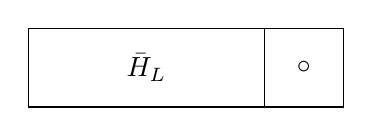
\begin{tikzpicture}
      \draw (0,.5) rectangle (3,-.5) node [midway] {$\bar H_L$};
      \draw (3,.5) rectangle (4,-.5) node [midway] {\ensuremath\circ};
    \end{tikzpicture}}_{H_{L+1}}
  \]
\end{enumerate}

\subsection{Eigenstates of the $\psi_i = 1$, $m$, $L$-site system}

S. White: Enlarge the system first, and add the boundary condition to the
enlarged system, which has less effect to the original system.
Then, project to the original system.
For non-interaction, the effect is pretty good.

But for the system with interaction, the result of the projection is
\[
  \ket|\Psi_{Sb}> 
  \begin{aligned}
    & \to \ket|\Psi_L^{(1)}>\\
    & \to \ket|\Psi_L^{(2)}>\\
  \end{aligned}, \qq{multiple numbers}
\]
and $\ket|\Psi_L^{(-)}>$ is the most proper one.
When executing the caclculation,
\[
  \underbrace{
  \underbrace{
  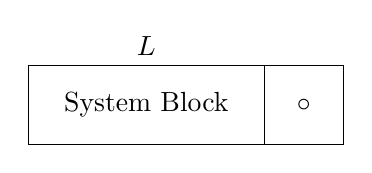
\begin{tikzpicture}
    \draw (0,.5) rectangle (3,-.5) node [midway] {System Block}
                 node [midway, above = .5cm] {$L$};
    \draw (3,.5) rectangle (4,-.5) node [midway] {\ensuremath\circ};
  \end{tikzpicture}}_{\text{$L+1$ System superblock}}
  \quad
  \underbrace{
  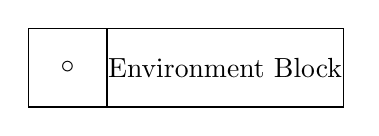
\begin{tikzpicture}
    \draw (0,.5) rectangle (3,-.5) node [midway] {Environment Block};
    \draw (-1,.5) rectangle (0,-.5) node [midway] {\ensuremath\circ};
  \end{tikzpicture}}_{\text{Environment superblock}}}_{\text{Superblock OBC}}
\]
\begin{enumext}
  \item Construct a basic state number and a superblock which needs exceed $m$
  but also small enough for exact diagonalization.
  \item Exactly diagnose the superblock, and take the lowest eigenstate ($m$)
  \item These states use system Sb basic state $\ket|i>$ and $CSb\ket|j>$
  \[
    \ket|\psi> = \sum_{ij} \psi_{ij} \ket|i>\ket|j>
  \]
  then project to the reduced density matrix of the sysbem Sb
  \[
    \rho_{ii'} = \sum_{j \text{(environment)}} \ketbra|\psi><\psi|
  \]
  where $\Tr\rho = 1$, then we can diagonalize $\rho$, the eigenvalues $W_\alpha \geq 0$, and $\sum_\alpha w_\alpha = 1$, and the eigenstates
  $\ket|u^\alpha>$.
  \item If $\alpha = 1$, $\ldots\,$,~$s$, then
  \begin{enumext}
    \item If $s \leq m$, then keep all the states;
    \item If $s > m$, them keep the $n$ maximum states of $w^\alpha$ in the $s$
    states.
  \end{enumext}
\end{enumext}

\begin{example}
  1D spin $\sfrac12$ AFM Heisenberg model
  \[
    H = \sum_i \bm S_i \bm S_{i+1}, \qq{let}
    m = S, S^z_\text{tot} = 0
  \]
  the so-called antiferromagnetic model.
  \begin{enumext}
    \item $L = 4$, the Superblock
    \[
      \underbrace{\underset{\text{Sys}}{\square}--
      \circ}_{\text{Sys Sb}}--\underbrace{\circ--
      \underset{\text{Cir}}{\square}}_{\text{Cir Sb}}
    \]
    contains $B_L$, $S_L$, $S_R$, $B_R$ respectively in the figure, and
    \begin{align*}
      & H_{B_L} = H_{S_L} = H_{S_R} = H_{B_R} = 0\\
      & S_{B_L}^z = S_{S_L}^z = S_{S_R}^z = S_{B_L}^z =
      \pdiagmat*{\sfrac12,\sfrac12}\\
      & S_{B_L}^+ = S_{S_L}^+ = S_{S_R}^+ = S_{B_L}^+ =
      \begin{psmallmatrix}
        0 & 1\\0 & 0
      \end{psmallmatrix}\\
      & S_{B_L}^- = \cdots =
      \begin{psmallmatrix}
        0 & 0\\1 & 0
      \end{psmallmatrix}
    \end{align*}
    The 4 blocks, to keep $S_\text{tot}^z = 0$, there are 6 states
    \[
      \ab(
        \begin{aligned}
        & \ket*|\frac12, \frac12, -\frac12, -\frac12>\\
        & \ket*|\frac12, -\frac12, \frac12, -\frac12>\\
        & \ket*|\frac12, -\frac12, -\frac12, \frac12>\\
        & \ket*|-\frac12, \frac12, \frac12, -\frac12>\\
        & \ket*|-\frac12, \frac12, -\frac12, \frac12>\\
        & \ket*|-\frac12, -\frac12, \frac12, \frac12>
        \end{aligned}
      )
    \]
    then, the Hamiltonian
    \[
      \hat H = \bm S_{B_L} \cdot \bm S_{S_L} + \bm S_{S_L} \cdot \bm S_{S_R}
            + \bm S_{S_R} \cdot \bm S_{B_R} =
      \begin{pmatrix}
        \frac14 & \frac12 & 0 & 0 & 0 & 0\\
        \frac12 & -\frac34 & \frac12 & \frac12 & 0 & 0\\
        0 & \frac12 & -\frac14 & 0 & \frac12 & 0\\
        0 & \frac12 & 0 & -\frac14 & \frac12 & 0\\
        0 & 0 & \frac12 & \frac12 & -\frac14 & \frac12\\
        0 & 0 & 0 & 0 & \frac12 & \frac12
      \end{pmatrix}
    \]
    The eigenvector
    \[
      \ket|\psi> =
      (0.149429, -0.557678, 0.408248, -0.557678, -.149427)\tran
    = \psi_{\frac12\frac12-\frac12\frac12-\frac12-\frac12} + \cdots
    \]
    and the density matrix element
    \[
      \rho_{i_1,i_2,i_1',i_2'}
    = \sum_{j_1j_2} \psi_{i_1i_2j_1j_2} \psi_{j_1j_2i_1'i_2'}
    \]
    from the basis
    \[
      \{\ket|i_1, i_2>\} =
      \{
        (\sfrac12,\sfrac12),
        (\sfrac12,-\sfrac12),
        (-\sfrac12,\sfrac12),
        (-\sfrac12,-\sfrac12)
      \}
    \]
    the density matrix is
    \[
      \rho = \begin{pmatrix}
        -0.022329 & 0 & 0 & 0\\
        0 & -0.477671 & 0.455342 & 0\\
        0 & 0.455342 & -0.477671 & 0\\
        0 & 0 & 0 & -0.022329
      \end{pmatrix}.
    \]
    Diagonalize $\rho$
    \[
      W = (0.022329, 0.933013, 0.022329, 0.022329)
    \]
    \[
      u^1 = (1,0,0,0)\tran,
      u^2 = (0,\sfrac{\sqrt2}{2},-\sfrac{\sqrt2}{2},0)\tran,
      u^3 = (0,\sfrac{\sqrt2}{2},\sfrac{\sqrt2}{2},0)\tran,
      u^4 = (0,0,0,1)\tran
    \]
    $S = 4\times 5$ matrix.
    \item $L = 2$.
  \end{enumext}
\end{example}

\section{K-T Phase Transition}

The spin on a 2D plane
\begin{equation}
  \bm S = (S_x, S_y), \qq{and}
  \mathcal H = -J'\sum_{\braket<ij>} \bm S_i \cdot \bm S_j
             = -\underbrace{J'S^2}_J \sum_{\braket<ij>}
              \cos(\theta_i - \theta_j)
\end{equation}
i.e., $X-Y$ model.
\begin{center}
  \begin{minipage}{.48\linewidth}
    \centering
    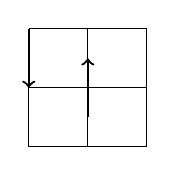
\begin{tikzpicture}[scale = .75]
      \draw (0,0) grid (2,2);
      \draw [thick, ->] (1,.5) --++ (0,1);
      \draw [thick, ->] (0,2) --++ (0,-1);
    \end{tikzpicture}
  \end{minipage}
  \hspace*\fill
  \begin{minipage}{.48\linewidth}
    \centering
    \begin{tikzpicture}
      \draw (0,0) -- (3.5,0);
      \draw [->, thick] (0,0) node [below] {$i$} --++ (1,.5)
       node [above] {$\bm S_i$};
      \draw [->, thick] (2,0) node [below] {$j$} --++ (.5,1)
       node [above] {$\bm S_j$};
    \end{tikzpicture}
  \end{minipage}
\end{center}
The partition function
\begin{equation}
  Z = \Tr \upe^{-\beta H} = \int_0^{2\pi} \prod_i \frac{\d\theta_i}{2\pi}
      \upe^{-\beta H(\theta_i)}
  \xlongequal{T \gg J/k_B}
    \int_0^{2\pi} \prod \frac{\d\theta_i}{2\pi} \prod_{\braket<ij>}
    (1 + \beta J\cos(\theta_i - \theta_j) + \mathcal O(\beta J)^2)
\end{equation}
Therefore
\begin{equation}
  \begin{aligned}
    \braket<\bm S_0 \cdot \bm S_1> & = S^2 \int_0^{2\pi}
    \prod_i \frac{\d\theta}{2\pi} \prod_{\braket<ij>}
    (1 + \beta J\cos(\theta_i - \theta_j))
    \cos(\theta_0 - \theta_i) \sim \ab(\frac{\beta J}{2})^{|\bm r|}\\
    & = \exp\ab(-\ln|\ab(\frac2{\beta J})^{|\bm r|}|)
    \equiv \exp\ab(-\frac{|\bm r|}{\xi})
  \end{aligned}
\end{equation}
where $\xi^{-1} = \ln\frac2{\beta J}$. The exponential state stands for the
disorder. This is so-called the \emph{High-temperature expansion.}

For \emph{Low-temperature expansion}, $\beta J \geq 1$.
It should near a ferronmagnetic state, so
$\theta_i - \theta_j \ll 1$,
$\cos(\theta_i - \theta_j) = 1 - \frac12(\theta_i - \theta_j)^2$.
\[
  (\theta_i - \theta_{i+\delta x})^2 + (\theta_i - \theta_{i+\delta y})^2
\Rightarrow a^2(\pdif x\theta_i)^2 + a^2(\pdif y\theta_i)^2
= a^2(\nabla \theta_i)^2
\]
At the continuous limit
\[
  \beta H = \beta E_0 - \frac{\beta J}{2} |\nabla\theta(x)|^2
\]
where $\beta E_0 = 2\beta JL^2/a^2$, $\braket<\cos(\theta_0-\theta_1)>
\sim |\bm r/a|^{-1/(2\pi\beta J)}$.
It is power low decay, we call it \emph{Quasi-long order}, or \emph{algebric},
or \emph{long range order}.

Take a peek $\fdv H\theta = 0$, then,
\[
  -(\nabla\theta)^2 = \theta\nabla^2\theta - \nabla(\theta\nabla\theta)
\]
we have $\nabla^2\theta = 0$.
\begin{enumext}
  \item $\theta = \text{Const}$
  \item $\nabla\theta = \ab(-\frac g{r^2}, \frac x{r^2})$,
        $\theta = \arctan(\frac yx)$, which satisfies
        $\oint \nabla\theta \d\bm r = 2\pi$
  \item Common solution: $\oint \nabla \theta \d\bm l = 2\pi n$
  
  The Hamiltonian
  \[
    H = -\theta \nabla^2\theta \to (\nabla\theta)^2
  \]
  where
  \[
    \nabla \theta \cdot \nabla\theta = \frac{x^2 + y^2}{r^4} = \frac1{r^2}
  \]
  Then, the integral
  \[
    \frac J2 \int \d^2 \bm r (\nabla\theta)^2 - E_0
  = \frac J2 \int_a^L r \d r \int_0^{2\pi} \d\theta \frac1{r^2}
  = J\pi \ln \frac La
  \]
  This kind of solution is a high-energy excitation at $T = 0$.

  Consider a pair of vertices: $\theta_1 - \theta_2 \approxeq 0$,
  $|\bm r_{12} \to \infty|$ with finite energy.
  \begin{center}
    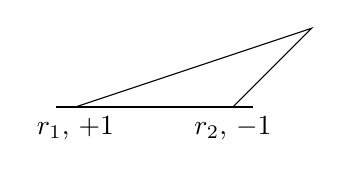
\begin{tikzpicture}
      \draw (-1.25,0) -- (1.25,0);
      \draw (-1,0) node [below] {$\bm r_1$, $+1$} -- (2,1) -- (1,0)
       node [below] {$\bm r_2$, $-1$};
    \end{tikzpicture}
  \end{center}
  \begin{align*}
    E_\text{vortex-pair} &
  = \int \d^2\bm r[(\nabla\theta_1)^2 + (\nabla\theta_2)^2]
  \approxeq \int_\text{core} \d^2\bm r(\nabla\theta_1)^2
            \int_\text{core} \d^2\bm r(\nabla\theta_2)^2\\
& = \int_a^R r \d r (\nabla\theta_1)^2 \d\theta +
    \int_a^R r\d r \d\theta (\nabla\theta_2)^2
  = 2E_\text{core} + 2J\pi\ln\frac Ra
  \end{align*}
  The 2D Column gas
  \[
    F = -\pdv ER = -\frac1R
  \]
  At a finite temperature, a vortex's square proportion to $a^2$.
  In a square of $L^2$, there can be around $L^2/a^2$ positions of vortices.
  The entropy
  \[
    S = \ln \ab(\frac{L^2}{a^2})
  \]
  then, the free energy of a vortex is
  \[
    F = U - TS = (J\pi\ln\frac La - T\ln\ab(\frac{L^2}{a^2}))
      = (J\pi - \frac2\beta) \ln\frac La
  \]
  If $J\pi - 2/\beta < 0$, then a single vortex can escape from the vortex-pair;
  and take a phase transition to becomes favorable.
  The critical temperature $T_c = J\pi/2k_B$.
\end{enumext}